\documentclass[a4paper]{article}

\usepackage[a4paper, top=8mm, bottom=8mm, left=8mm, right=8mm]{geometry}
\usepackage{float}
\usepackage{graphicx}

\usepackage{polyglossia}
\setdefaultlanguage[babelshorthands=true]{russian}
\setotherlanguage{english}

\usepackage{fontspec}
\setmainfont{FreeSerif}
\newfontfamily{\russianfonttt}[Scale=0.7]{DejaVuSansMono}

\usepackage[tiny, compact]{titlesec}

\usepackage{titling}
\setlength{\droptitle}{-1cm}
\pretitle{\begin{center}\begin{bfseries}\Large}
\posttitle{\par\end{bfseries}\end{center}}
\preauthor{\begin{center}\normalsize}
\postauthor{\par\end{center}\vspace{-1.8cm}}

\usepackage{hyperref}
\usepackage{bookmark}
\usepackage{csquotes}
\usepackage{booktabs}
\usepackage{multirow}

\title{Сравнение форматов хранения разреженных матриц: COO и QuadTree}

\author{Нарышев Сергей Иванович}

\date{}

\begin{document}

\maketitle

\begin{flushright}
    Группа: \emph{2025.Б-72-мм}

    Кафедра: \emph{кафедра системного программирования}

    Научный руководитель: \emph{Григорьев Семён Вячеславович}

    Номер семестра практики: \emph{2}
\end{flushright}

\section{Введение}

Разреженные матрицы~--- матрицы, в которых большинство элементов равны нулю,~--- встречаются повсеместно: в задачах вычислительной математики, анализе графов, обработке изображений и машинном обучении. Хранить такую матрицу в плотном формате~--- двумерном массиве~--- неэффективно: память тратится на нули, а операции над матрицей вынуждены обходить бесполезные элементы.

Существует множество форматов компактного хранения разреженных матриц. Среди наиболее распространённых~--- CSR (Compressed Sparse Row), CSC (Compressed Sparse Column) и COO (Coordinate List). CSR и CSC оптимизированы для последовательного доступа к строкам или столбцам, но предполагают статичную структуру: добавление или удаление элементов требует перестроения внутренних массивов. COO~--- простейший формат, в котором каждый ненулевой элемент задаётся тройкой (строка, столбец, значение). Он удобен для построения матрицы и передачи данных между библиотеками, но неэффективен для произвольного доступа: поиск элемента требует перебора списка.

В проекте QTreeFSharp~\footnote{URL: \url{https://github.com/Lamagraph/QTreeFSharp} (дата обращения: 15.07.2026).} используется альтернативный подход~--- дерево квадрантов (quadtree). Матрица представляется бинарным деревом, каждый внутренний узел которого содержит четыре поддерева, соответствующих четвертям матрицы. Если все четыре поддерева одинаковы, они сжимаются в один лист. Такая структура естественным образом обеспечивает разреженное хранение и позволяет эффективно выполнять рекурсивные операции (умножение матриц, отображение, свёртку), поскольку операция применяется только к занятым поддеревьям.

QTreeFSharp~--- это библиотека разреженных векторов и матриц на языке F\#~\footnote{URL: \url{https://en.wikibooks.org/wiki/F_Sharp_Programming} (дата обращения: 15.07.2026).}, реализующая базовые операции линейной алгебры и алгоритмы анализа графов в парадигме GraphBLAS~--- модели вычислений, в которой линейная алгебра используется как язык для работы с графами.

\section{Постановка задачи}

В исходном проекте единственным форматом хранения разреженных матриц был quadtree. Формат COO отсутствовал. Это создавало неудобства при импорте данных: многие библиотеки (SuiteSparse, SciPy, MATLAB) используют CSR или COO как формат обмена, а конвертация требовала промежуточных преобразований.

Кроме того, не было данных о том, как quadtree сравнивается с традиционными форматами по производительности. Для одних операций (доступ по индексу, умножение матриц) дерево может оказываться быстрее за счёт кэширования и сокращения числа обходимых элементов, для других (построение, обновление)~--- медленнее из-за накладных расходов рекурсии и аллокаций.

\section{Цель работы}

Целью работы является реализация формата COO (Coordinate List) для хранения разреженных матриц в библиотеке QTreeFSharp и сравнение его производительности с существующим форматом quadtree на синтетических и реальных данных.

\section{Задачи работы}

Для достижения цели были поставлены следующие задачи.

\begin{enumerate}
    \item Реализовать модуль COO с базовыми операциями: доступ к элементу (\texttt{cooGet}), обновление элемента (\texttt{cooUpdate}), отображение (\texttt{cooMap}, \texttt{cooMapi}), поэлементное отображение двух матриц (\texttt{cooMap2}, \texttt{cooMap2i}) и умножение матриц (\texttt{mxmcoo}).
    \item Реализовать мостовые функции для конвертации между форматами COO и quadtree (\texttt{fromCoordinateList}, \texttt{toCoordinateList}).
    \item Написать модульные тесты для проверки корректности реализованных операций.
    \item Разработать инфраструктуру измерения производительности на базе BenchmarkDotNet для сравнения двух форматов.
    \item Провести измерения на синтетических данных (разреженных и плотных матрицах различных размеров).
    \item Провести измерения на реальных матрицах из коллекции SuiteSparse~\footnote{URL: \url{https://sparse.tamu.edu/} (дата обращения: 15.07.2026).}.
\end{enumerate}

\section{Актуальность и область применения}

Разреженные матрицы составляют основу большинства задач вычислительной линейной алгебры. Выбор формата хранения напрямую влияет на скорость выполнения и потребление памяти. Результаты сравнительного анализа полезны разработчикам библиотек линейной алгебры и вычислительных пакетов при выборе внутреннего представления данных.

Проект QTreeFSharp является прототипом реализации вычислений с помощью interaction nets~--- формальной модели параллельных вычислений. Сравнение с традиционным форматом COO позволяет понять, какие операции целесообразно реализовывать на деревьях квадрантов, а какие~--- на плоских структурах данных.

\section{Описание решения}

\subsection{Формат COO}

Формат COO (Coordinate List)~--- простейший формат хранения разреженных матриц. Каждый ненулевой элемент матрицы представляется тройкой: номер строки, номер столбца и значение. Все тройки хранятся в упорядоченном списке.

В библиотеке QTreeFSharp формат COO реализован в модуле \texttt{COO}. Основной тип~--- \texttt{CoordinateList}, содержащий количество строк, количество столбцов и список троек \texttt{COOEntry}. Типы строк и столбцов помечены единицами измерения F\# (\texttt{rowindex}, \texttt{colindex}), что позволяет системе типов предотвратить смешивание индексов разных размерностей.

Операции над матрицей в формате COO:

\begin{itemize}
    \item \texttt{cooGet}~--- поиск элемента по индексу. Выполняет линейный перебор списка троек до нахождения нужной позиции или достижения конца списка. Сложность в худшем случае~--- $O(n)$, где $n$~--- число ненулевых элементов.
    \item \texttt{cooUpdate}~--- обновление значения элемента. Список троек поддерживается в отсортированном порядке; при обновлении элемент вставляется на нужную позицию. Реализация использует итеративный алгоритм с двумя циклами: первый~--- поиск позиции и копирование элементов до неё, второй~--- копирование оставшихся элементов.
    \item \texttt{cooMap}~--- применение функции к каждому элементу. Если функция возвращает \texttt{None} для отсутствующих элементов (нормальный режим), обрабатываются только существующие тройки. Если функция возвращает значение для отсутствующих элементов, выполняется полный перебор всех позиций матрицы~--- этот режим используется редко и работает медленнее.
    \item \texttt{cooMapi}~--- аналог \texttt{cooMap}, но функция получает также индексы строки и столбца.
    \item \texttt{cooMap2}, \texttt{cooMap2i}~--- поэлементное отображение двух матриц. Списки троек обеих матриц проходятся одновременно; при совпадении индексов функция получает оба значения, при несовпадении~--- только одно.
    \item \texttt{mxmcoo}~--- умножение матриц. Реализовано два алгоритма: оптимизированный (группировка по строкам для операций, поглощающих \texttt{None}) и общий (полный перебор всех комбинаций строк и столбцов).
\end{itemize}

\subsection{Формат QuadTree}

В формате quadtree матрица представляется деревом типа \texttt{qtree}. Лист (\texttt{Leaf}) содержит либо \texttt{Dummy} (пустая область), либо \texttt{UserValue(Some v)} (ненулевой элемент) или \texttt{UserValue(None)} (область, заполненная нулями). Внутренний узел (\texttt{Node}) содержит четыре поддерева: NW (северо-запад), NE (северо-восток), SW (юго-запад), SE (юго-восток).

Ключевой механизм~--- конденсация: если после операции все четыре потомка узла оказались одинаковыми листьями, они сливаются в один. Это обеспечивает компактность структуры для данных с повторяющимися блоками.

Операции над матрицей в формате quadtree:

\begin{itemize}
    \item \texttt{get}~--- доступ к элементу. Выполняется рекурсивный спуск по дереву: на каждом уровне определяется, в какой квадрант попадает искомый индекс, и выбирается соответствующее поддерево. Сложность~--- $O(\log N)$, где $N$~--- размер стороны матрицы.
    \item \texttt{set}~--- обновление элемента. Аналогичный рекурсивный спуск с заменой листа на нужной глубине и пересчётом числа ненулевых элементов. Возвращает новую матрицу (функциональная немутабельность).
    \item \texttt{map}, \texttt{mapi}~--- рекурсивное отображение с обходом только занятых поддеревьев.
    \item \texttt{map2}, \texttt{map2i}~--- рекурсивное отображение двух матриц, совмещённых по структуре дерева.
    \item \texttt{mxm}~--- умножение матриц по алгоритму divide-and-conquer: матрица делится на четыре подматрицы, выполняются восемь рекурсивных умножений и четыре сложения подматриц.
\end{itemize}

\subsection{Мостовые функции}

Для конвертации между форматами реализованы две функции:

\begin{itemize}
    \item \texttt{fromCoordinateList}~--- преобразование COO в quadtree. Список троек рекурсивно разделяется на четыре квадранта, строится дерево с последующей конденсацией.
    \item \texttt{toCoordinateList}~--- преобразование quadtree в COO. Рекурсивный обход дерева, собирающий все листья с ненулевыми значениями в список троек.
\end{itemize}

\section{Модульные тесты}

Для проверки корректности реализованных операций написаны модульные тесты с использованием фреймворка xUnit. Всего написано 133 теста, из которых 27~--- для модуля COO. Тесты покрывают:

\begin{itemize}
    \item \texttt{cooGet}: поиск существующего элемента, отсутствующего элемента и обращение за пределы матрицы.
    \item \texttt{cooUpdate}: вставка нового элемента, обновление существующего, вставка в начало и конец списка.
    \item \texttt{cooMap} и \texttt{cooMapi}: отображение с сохранением и удалением элементов, а также полный режим с заполнением отсутствующих позиций (в том числе с зависящей от индексов функцией).
    \item \texttt{cooMap2} и \texttt{cooMap2i}: поэлементное отображение совпадающих и несовпадающих матриц.
    \item \texttt{mxmcoo}: умножение матриц с различными операциями сложения и умножения, включая случай, когда операция умножения поглощает \texttt{None} (оптимизированный путь), и случай, когда не поглощает (общий путь).
    \item Границы: пустые матрицы, матрицы нулевого размера, матрицы размером $1 \times 1$, матрицы с одним ненулевым элементом.
\end{itemize}

Все 133 теста проходят успешно.

\section{Экспериментальная оценка}

\subsection{Инструменты и окружение}

Измерения проводились с использованием BenchmarkDotNet~\footnote{URL: \url{https://benchmarkdotnet.org/} (дата обращения: 15.07.2026).}~--- фреймворка для микробенчмарков .NET. Среда исполнения~--- .NET 10. Операционная система~--- Windows 11. Процессор~--- AMD Ryzen 7 5800HS (3.20\,ГГц, 8 физических ядер, 16 логических). Каждая операция выполнялась в профиле \emph{ShortRun}: один запуск (LaunchCount=1) с тремя прогревочными и тремя измеряемыми итерациями; для запуска BenchmarkDotNet вычисляет математическое ожидание времени (Mean) и стандартное отклонение (StdDev). Для синтетических разреженных и реальных матриц операции \texttt{map}, \texttt{get}, \texttt{set} и \texttt{mxm} измерялись в пяти независимых запусках; итоговое значение~--- среднее по пяти запускам с межзапусковым стандартным отклонением. Операция \texttt{mapi} была переизмерена после доработки реализации \texttt{cooMapi} также в пяти запусках. Для плотных матриц ввиду высокой стоимости измерений (отдельные комбинации требуют десятков секунд на итерацию) каждая комбинация измерялась в одном запуске; для таких данных межзапусковое отклонение не вычислялось.

Визуализация результатов выполнялась с помощью Matplotlib~\footnote{URL: \url{https://matplotlib.org/stable/contents.html} (дата обращения: 15.07.2026).}.

\subsection{Эксперимент~1: Синтетические разреженные матрицы}

Сгенерированы синтетические квадратные матрицы трех размеров: $256 \times 256$, $512 \times 512$ и $1024 \times 1024$. Плотность заполнения~--- 1\% и 5\% (доля ненулевых элементов). Матрицы случайным образом заполнялись ненулевыми значениями.

Сравнивались операции: \texttt{map} (отображение), \texttt{mapi} (отображение с индексами), \texttt{get} (доступ к элементу), \texttt{set} (обновление элемента), \texttt{mxm} (умножение матриц).

На рис.~\ref{fig:sparse_map_1}--\ref{fig:sparse_get_1} приведены результаты для матриц с плотностью~1\%.

\begin{figure}[H]
    \centering
    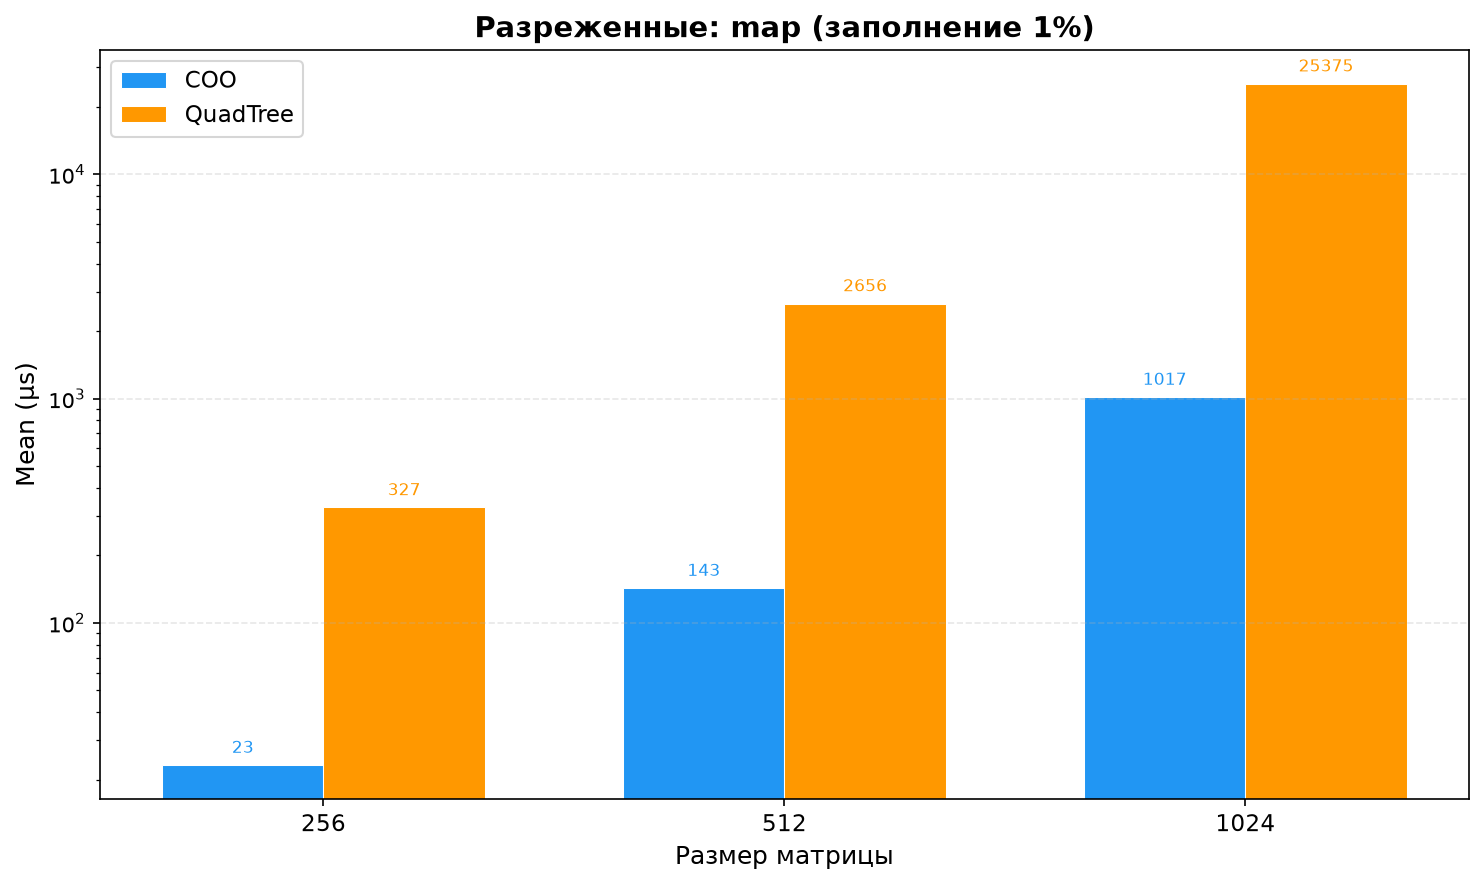
\includegraphics[width=0.92\textwidth]{images/sparse_map_fill1.png}
    \caption{Время выполнения \texttt{map} на синтетических разреженных матрицах (плотность~1\%). Ось~Y~--- время в микросекундах (логарифмическая шкала).}
    \label{fig:sparse_map_1}
\end{figure}

\begin{figure}[H]
    \centering
    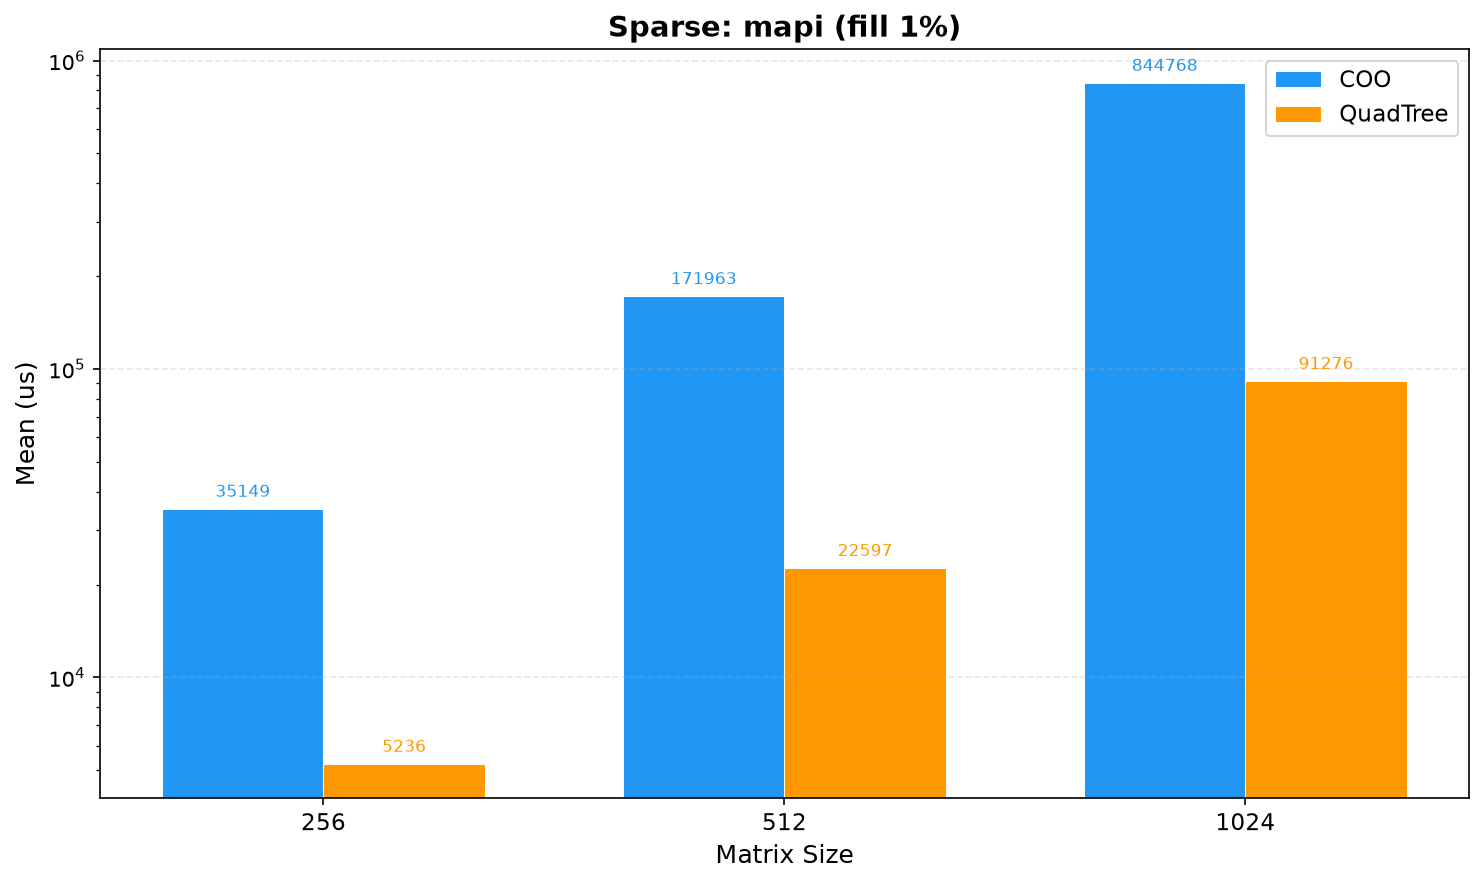
\includegraphics[width=0.92\textwidth]{images/sparse_mapi_fill1.png}
    \caption{Время выполнения \texttt{mapi} на синтетических разреженных матрицах (плотность~1\%).}
    \label{fig:sparse_mapi_1}
\end{figure}

\begin{figure}[H]
    \centering
    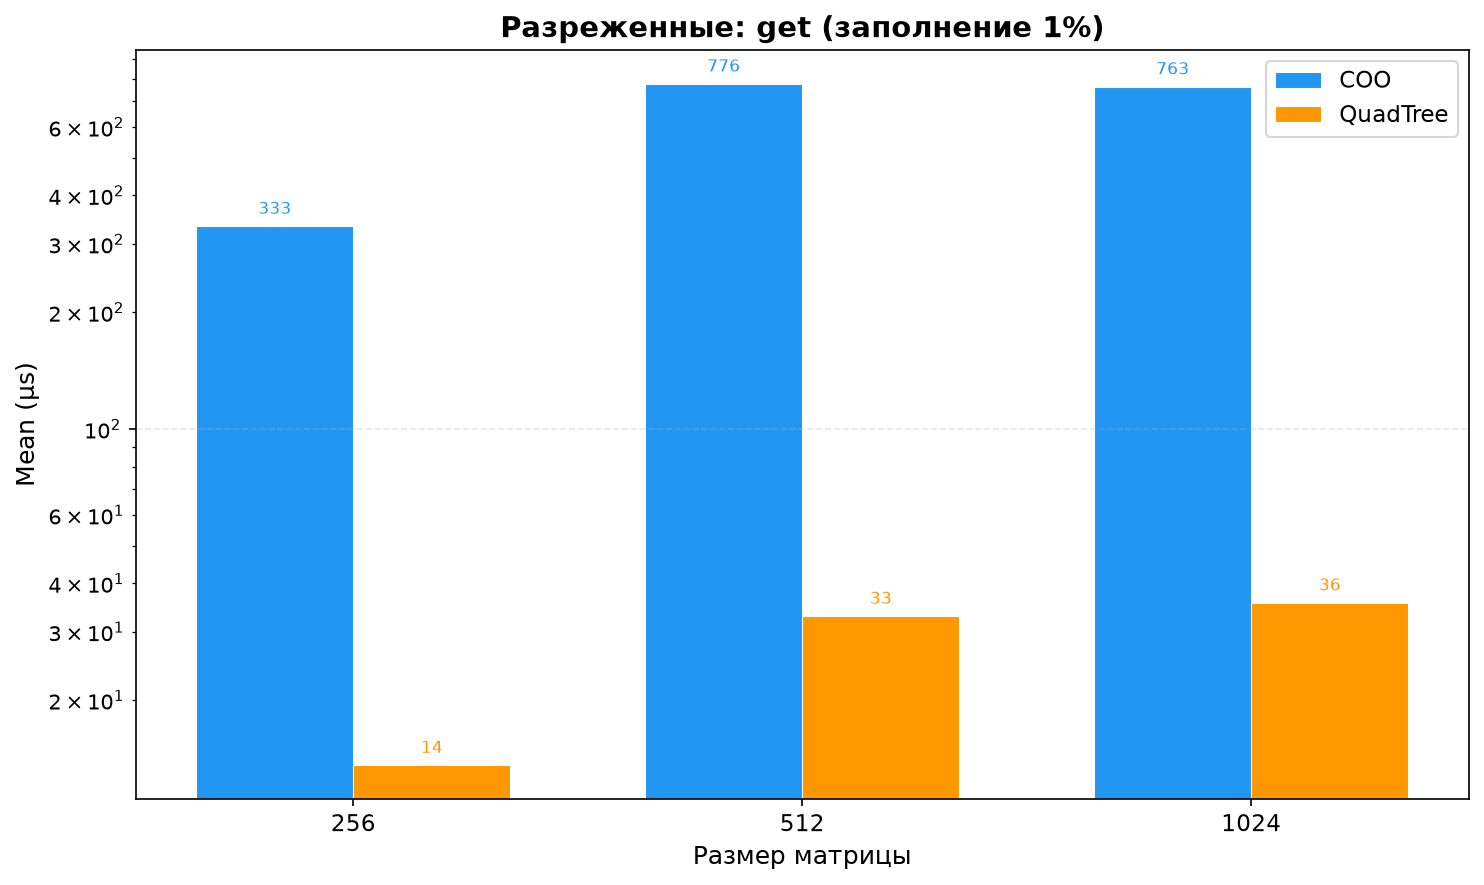
\includegraphics[width=0.92\textwidth]{images/sparse_get_fill1.png}
    \caption{Время выполнения \texttt{get} на синтетических разреженных матрицах (плотность~1\%).}
    \label{fig:sparse_get_1}
\end{figure}

\begin{figure}[H]
    \centering
    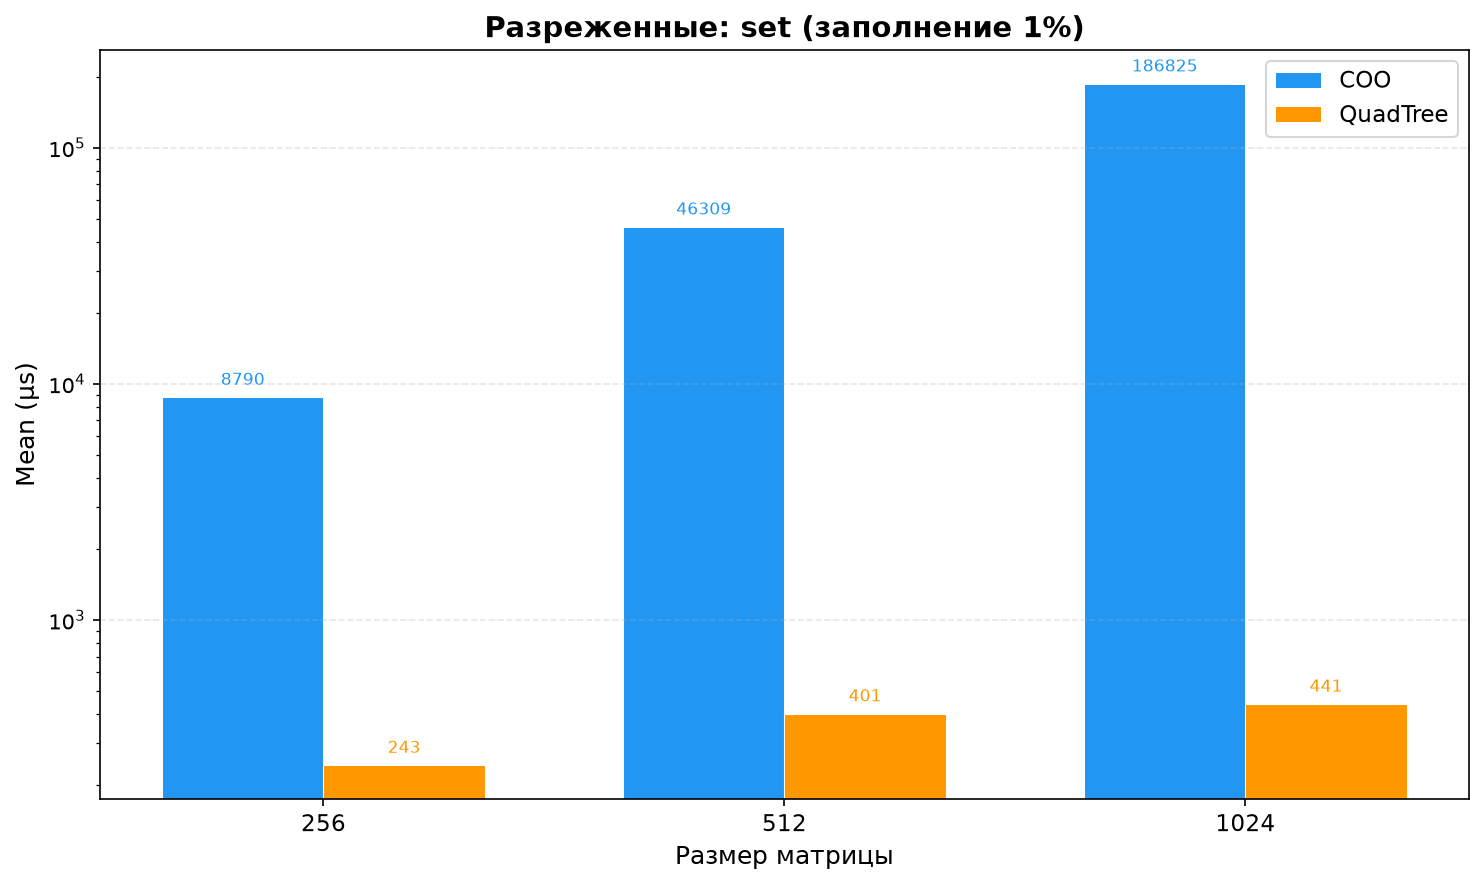
\includegraphics[width=0.92\textwidth]{images/sparse_set_fill1.png}
    \caption{Время выполнения \texttt{set} на синтетических разреженных матрицах (плотность~1\%).}
    \label{fig:sparse_set_1}
\end{figure}

\begin{figure}[H]
    \centering
    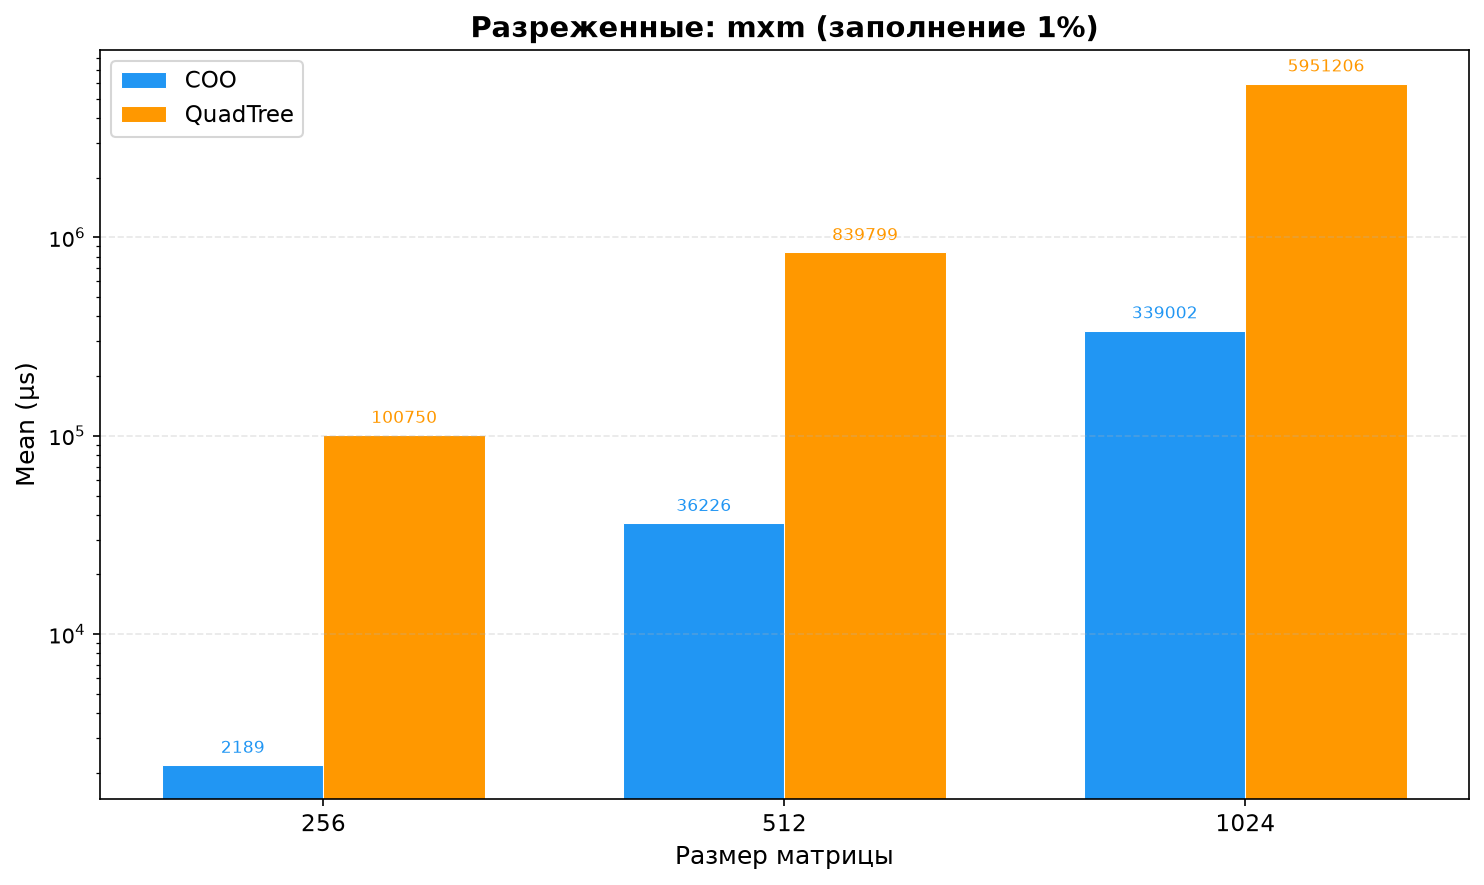
\includegraphics[width=0.92\textwidth]{images/sparse_mxm_fill1.png}
    \caption{Время выполнения \texttt{mxm} на синтетических разреженных матрицах (плотность~1\%).}
    \label{fig:sparse_mxm_1}
\end{figure}

\begin{figure}[H]
    \centering
    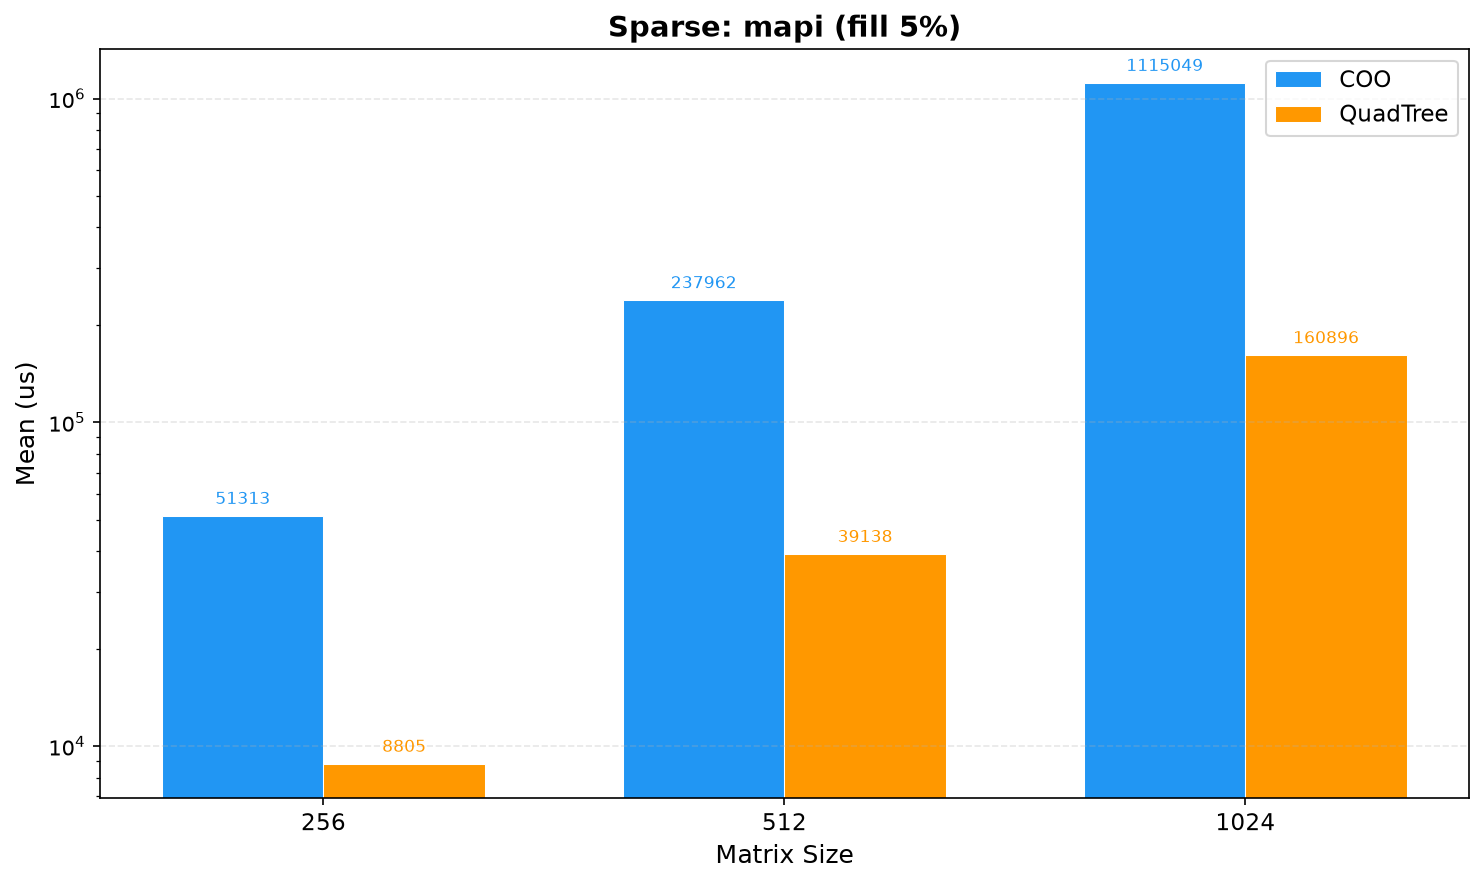
\includegraphics[width=0.92\textwidth]{images/sparse_mapi_fill5.png}
    \caption{Время выполнения \texttt{mapi} на синтетических разреженных матрицах (плотность~5\%).}
    \label{fig:sparse_mapi_5}
\end{figure}

Результаты для матриц с плотностью~5\% аналогичны по характеру для остальных операций, но абсолютные значения времени выше пропорционально числу ненулевых элементов.

\subsection{Эксперимент~2: Плотные матрицы}

Для оценки поведения форматов при максимальной нагрузке проведены измерения на полностью заполненных матрицах размеров $64 \times 64$, $128 \times 128$ и $256 \times 256$. Результаты приведены на рис.~\ref{fig:dense_map}--\ref{fig:dense_mxm}.

\begin{figure}[H]
    \centering
    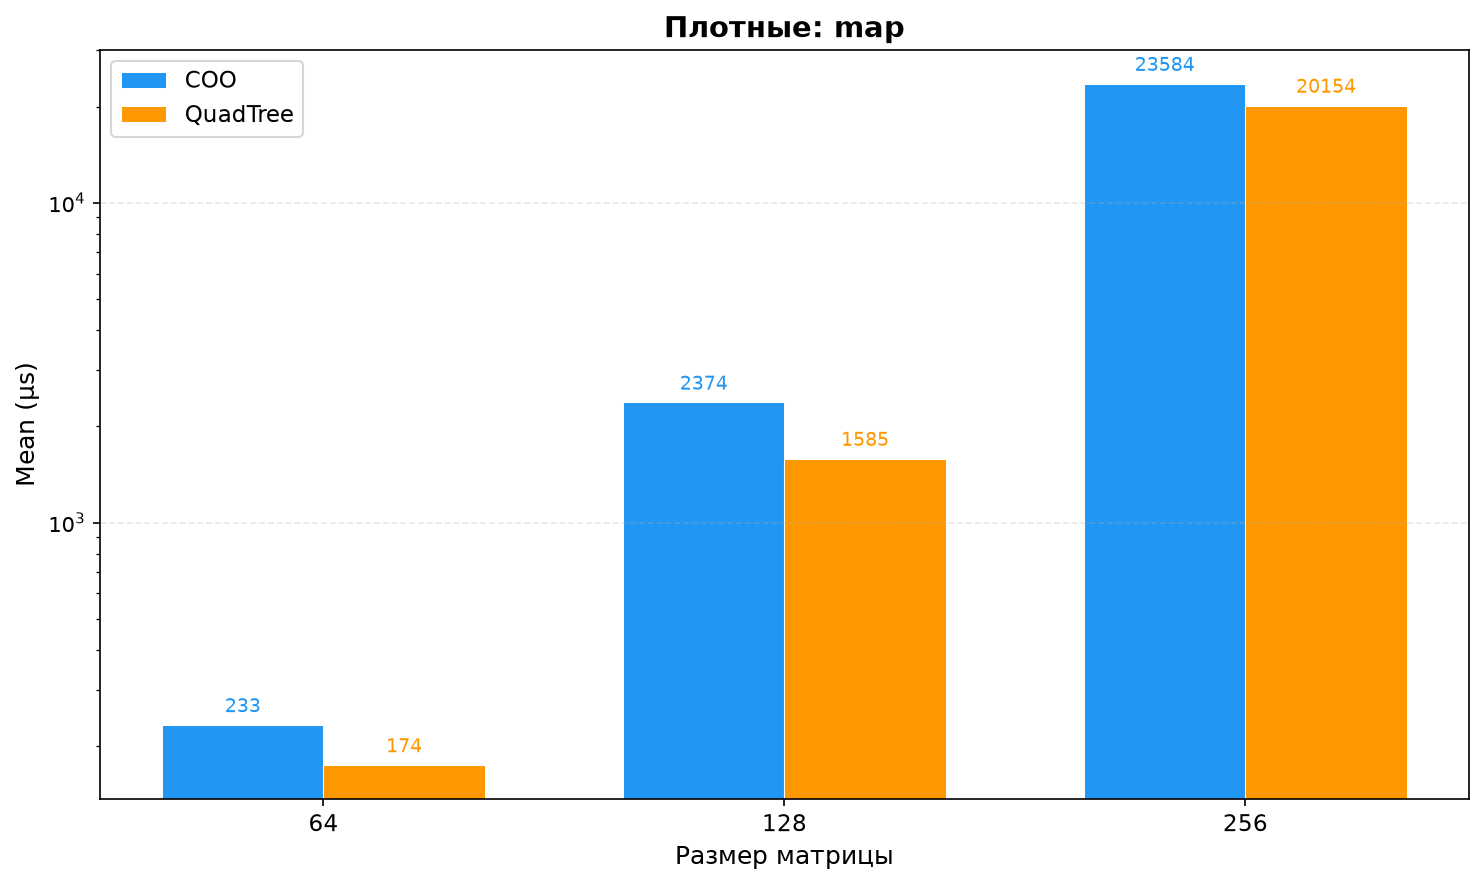
\includegraphics[width=0.92\textwidth]{images/dense_map.png}
    \caption{Время выполнения \texttt{map} на плотных матрицах. Ось~Y~--- время в микросекундах (логарифмическая шкала).}
    \label{fig:dense_map}
\end{figure}

\begin{figure}[H]
    \centering
    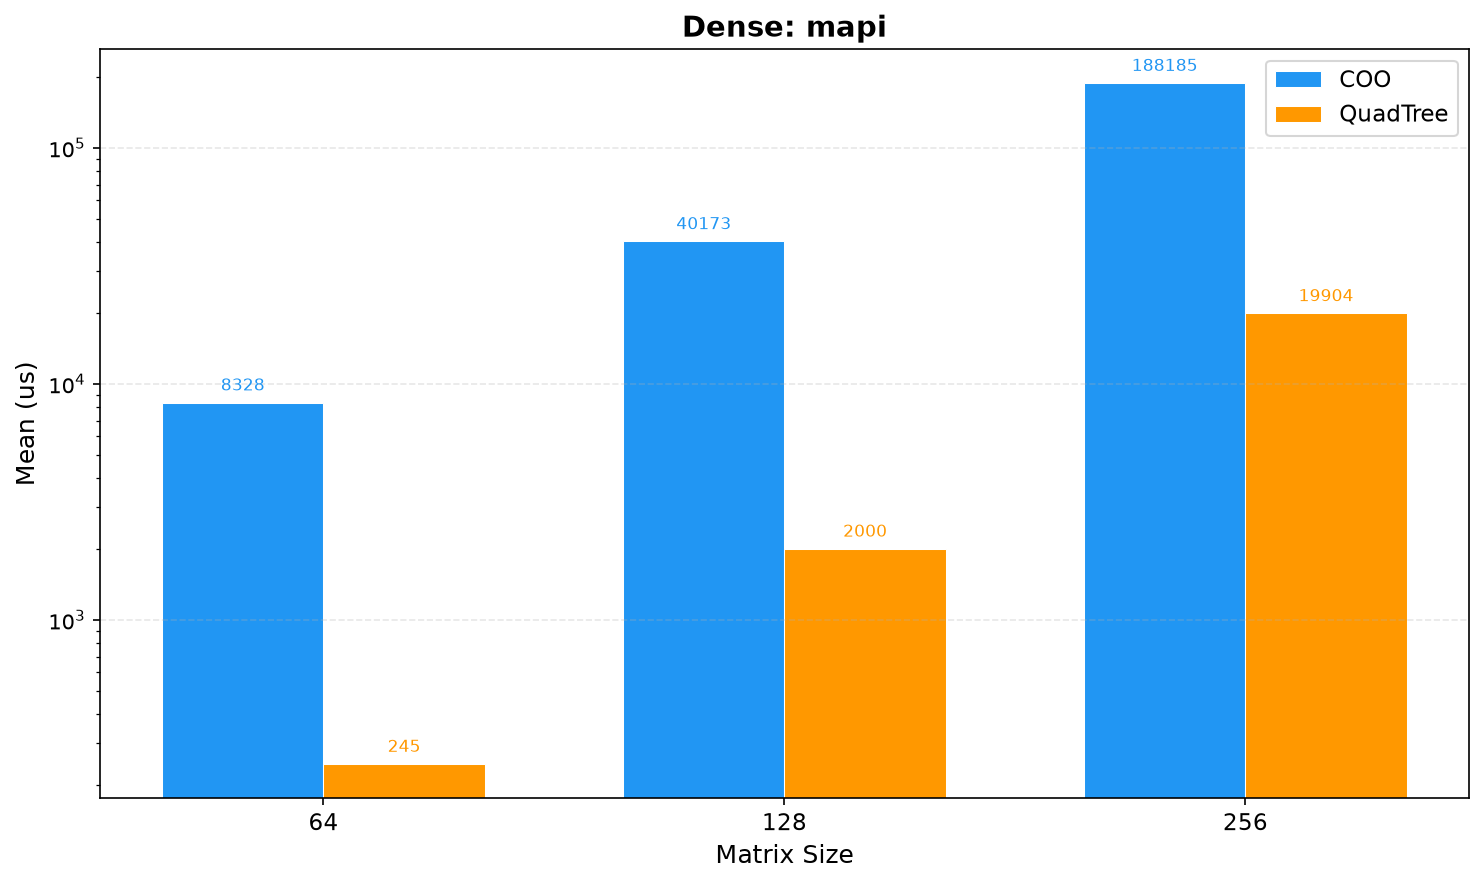
\includegraphics[width=0.92\textwidth]{images/dense_mapi.png}
    \caption{Время выполнения \texttt{mapi} на плотных матрицах.}
    \label{fig:dense_mapi}
\end{figure}

\begin{figure}[H]
    \centering
    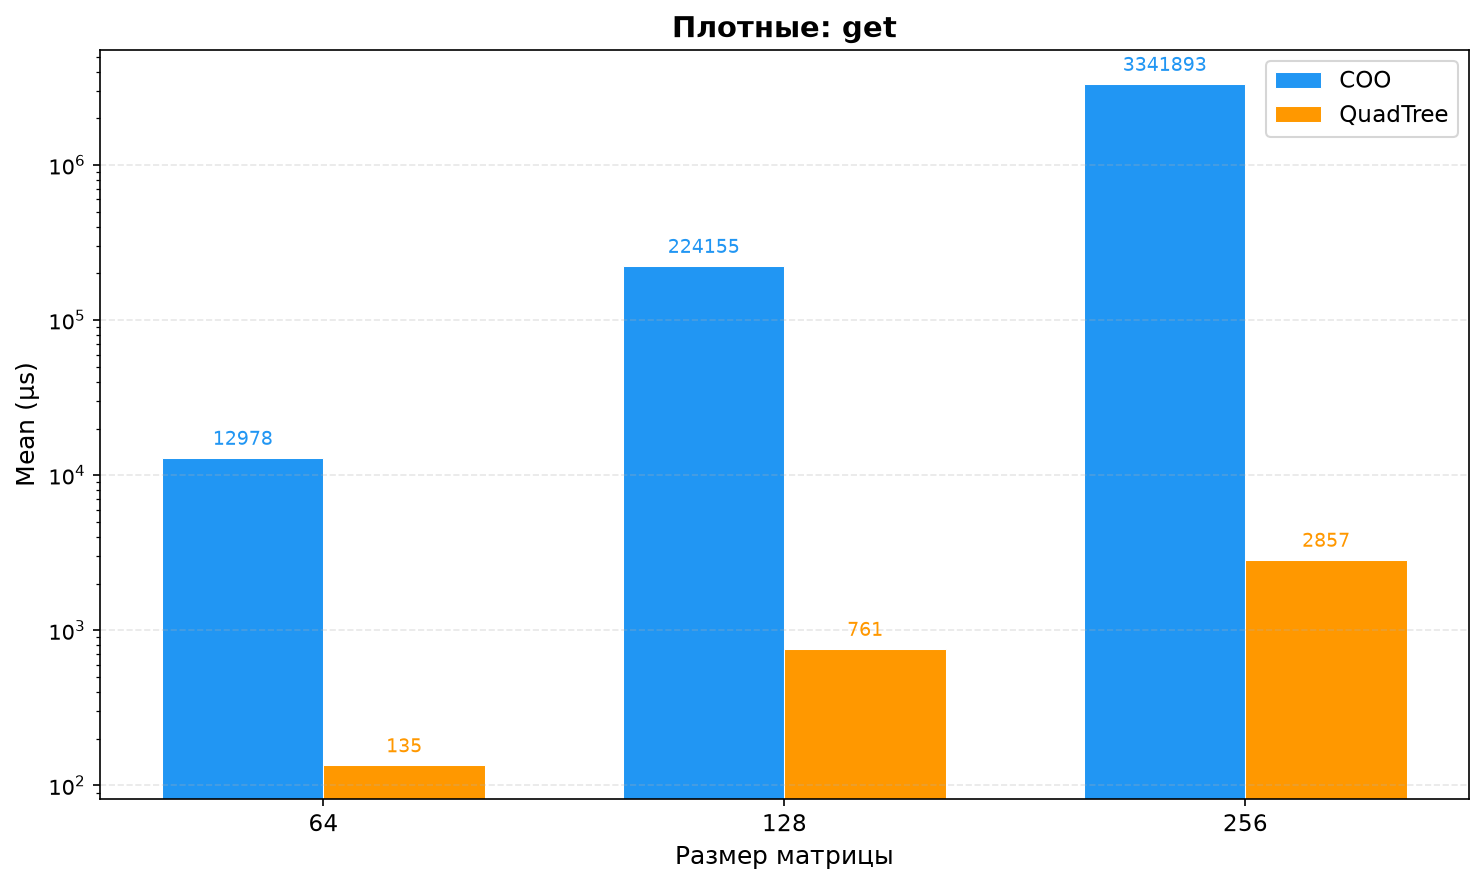
\includegraphics[width=0.92\textwidth]{images/dense_get.png}
    \caption{Время выполнения \texttt{get} на плотных матрицах.}
    \label{fig:dense_get}
\end{figure}

\begin{figure}[H]
    \centering
    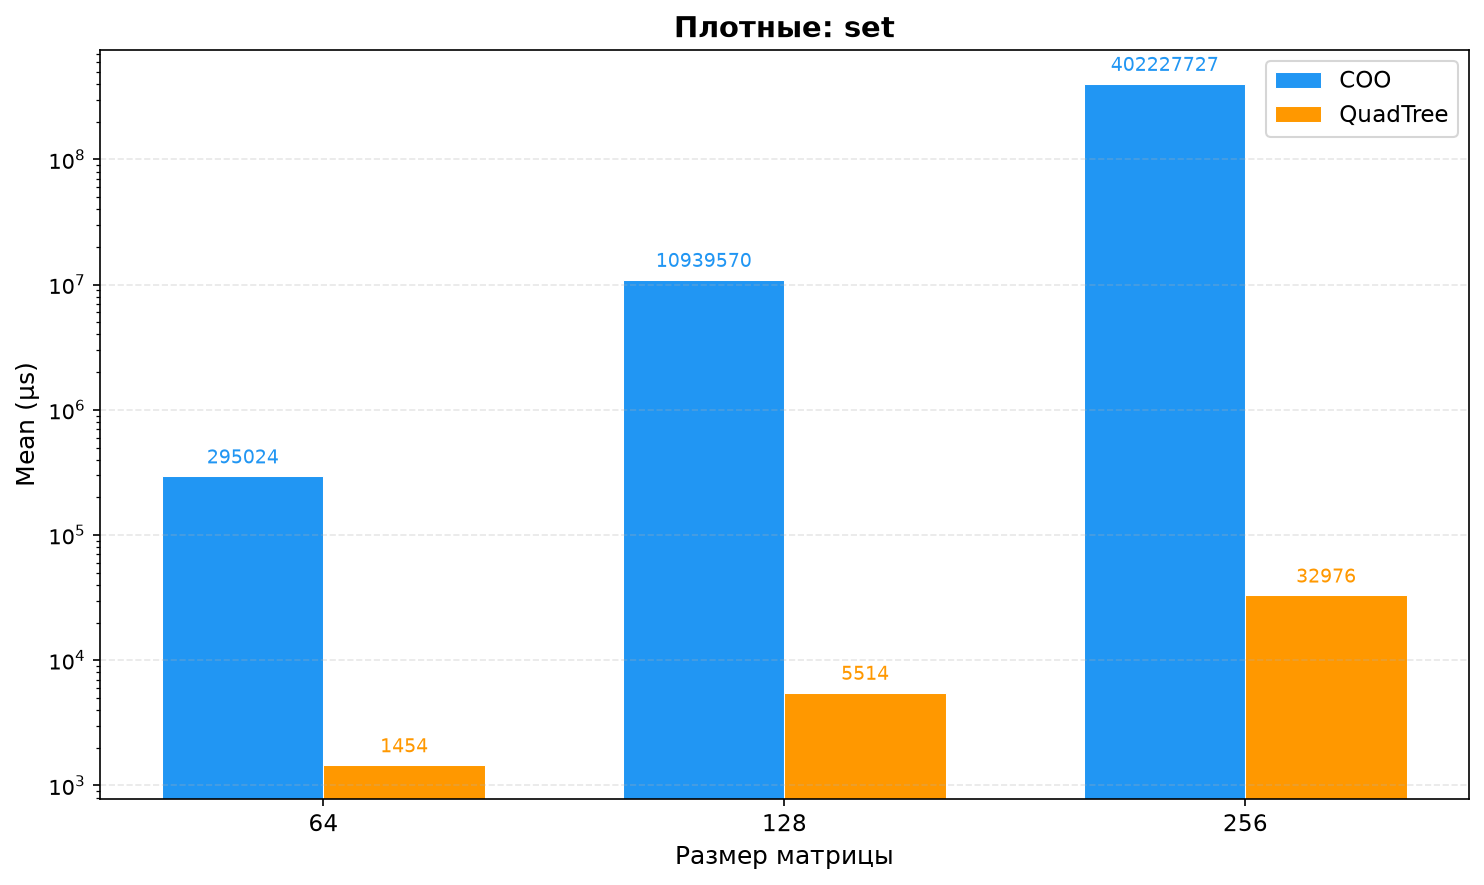
\includegraphics[width=0.92\textwidth]{images/dense_set.png}
    \caption{Время выполнения \texttt{set} на плотных матрицах.}
    \label{fig:dense_set}
\end{figure}

\begin{figure}[H]
    \centering
    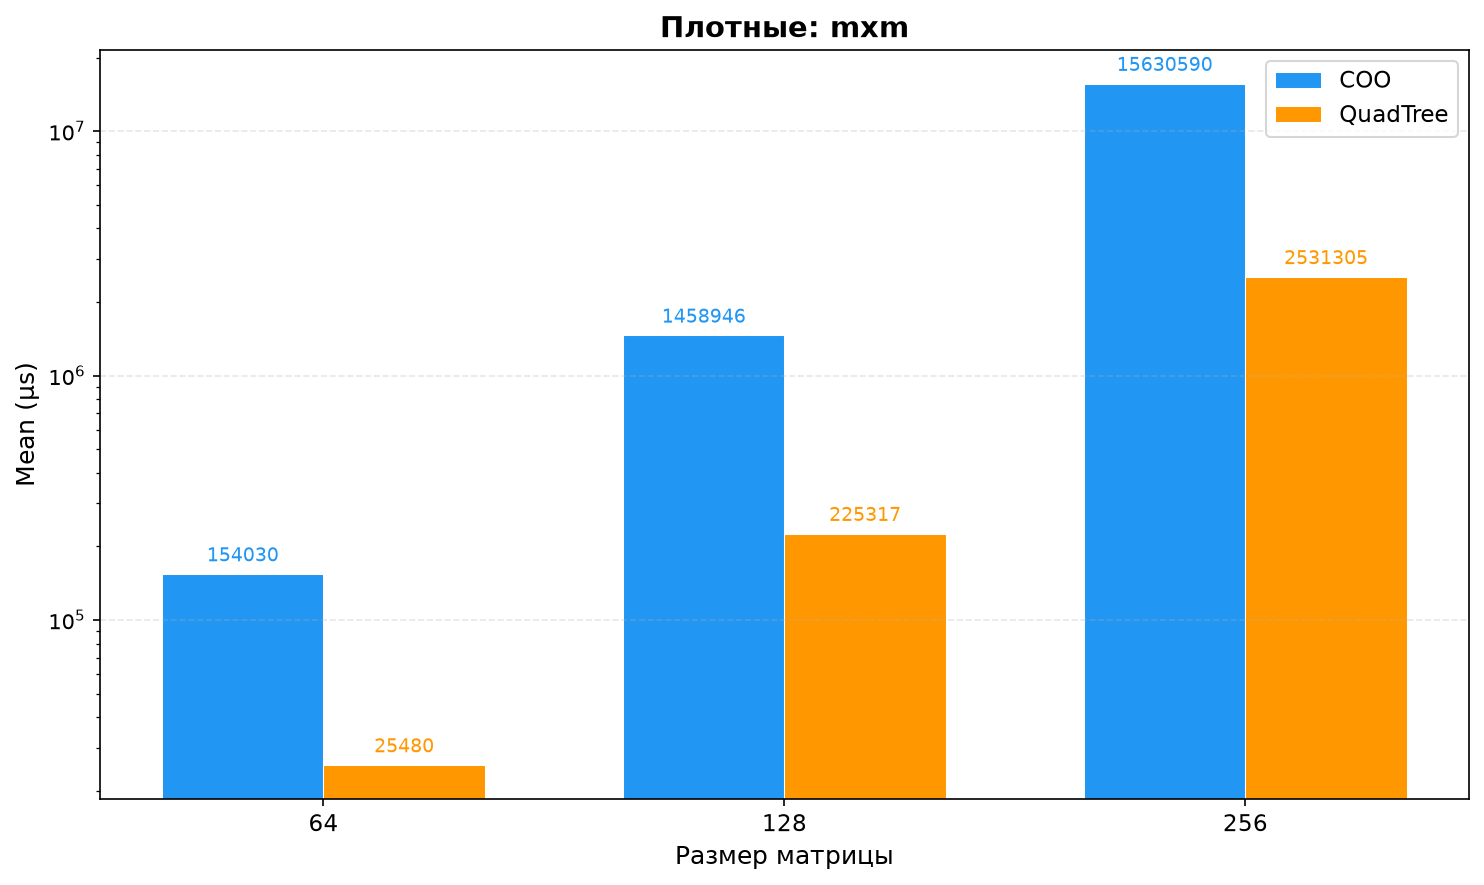
\includegraphics[width=0.92\textwidth]{images/dense_mxm.png}
    \caption{Время выполнения \texttt{mxm} на плотных матрицах.}
    \label{fig:dense_mxm}
\end{figure}

На плотных данных quadtree оказывается быстрее COO во всех измеряемых операциях. В операции \texttt{map} преимущество достигается за счёт того, что рекурсивный обход дерева затрагивает только листья, а разница оказывается небольшой (на размере $256 \times 256$ COO~--- 23.6\,мс, quadtree~--- 20.2\,мс). Операция \texttt{mapi} в COO требует полного перебора всех $N^2$ позиций, поэтому на плотных матрицах COO заметно медленнее: на $256 \times 256$~--- 188\,мс против 19.9\,мс у quadtree (в ~9.5 раза). В операции \texttt{get} quadtree обходит лишь $\log N$ уровней дерева, тогда как COO~--- линейный перебор списка, что даёт разрыв в тысячи раз. Операция \texttt{set} в COO вынуждена пересоздавать отсортированный список при каждом обновлении, из-за чего на $256 \times 256$ время достигает ~400\,с против ~33\,мс у quadtree.

\subsection{Эксперимент~3: Реальные матрицы}

Для оценки производительности на данных реальной структуры использовались матрицы из коллекции SuiteSparse Matrix Collection~--- крупнейшей базы данных разреженных матриц, применяемых в вычислительной математике. Загружены две матрицы:

\begin{itemize}
    \item \textbf{494\_bus}~--- матрица размера $494 \times 494$ с 1620 ненулевыми элементами (из задач моделирования энергосистемы).
    \item \textbf{arc130}~--- матрица размера $130 \times 130$ с 314 ненулевыми элементами (из аэрокосмической задачи).
\end{itemize}

Матрицы были загружены в формате Matrix Market и преобразованы в оба внутренних формата: COO и quadtree. Результаты приведены на рис.~\ref{fig:real_summary}--\ref{fig:real_mxm}.

\begin{figure}[H]
    \centering
    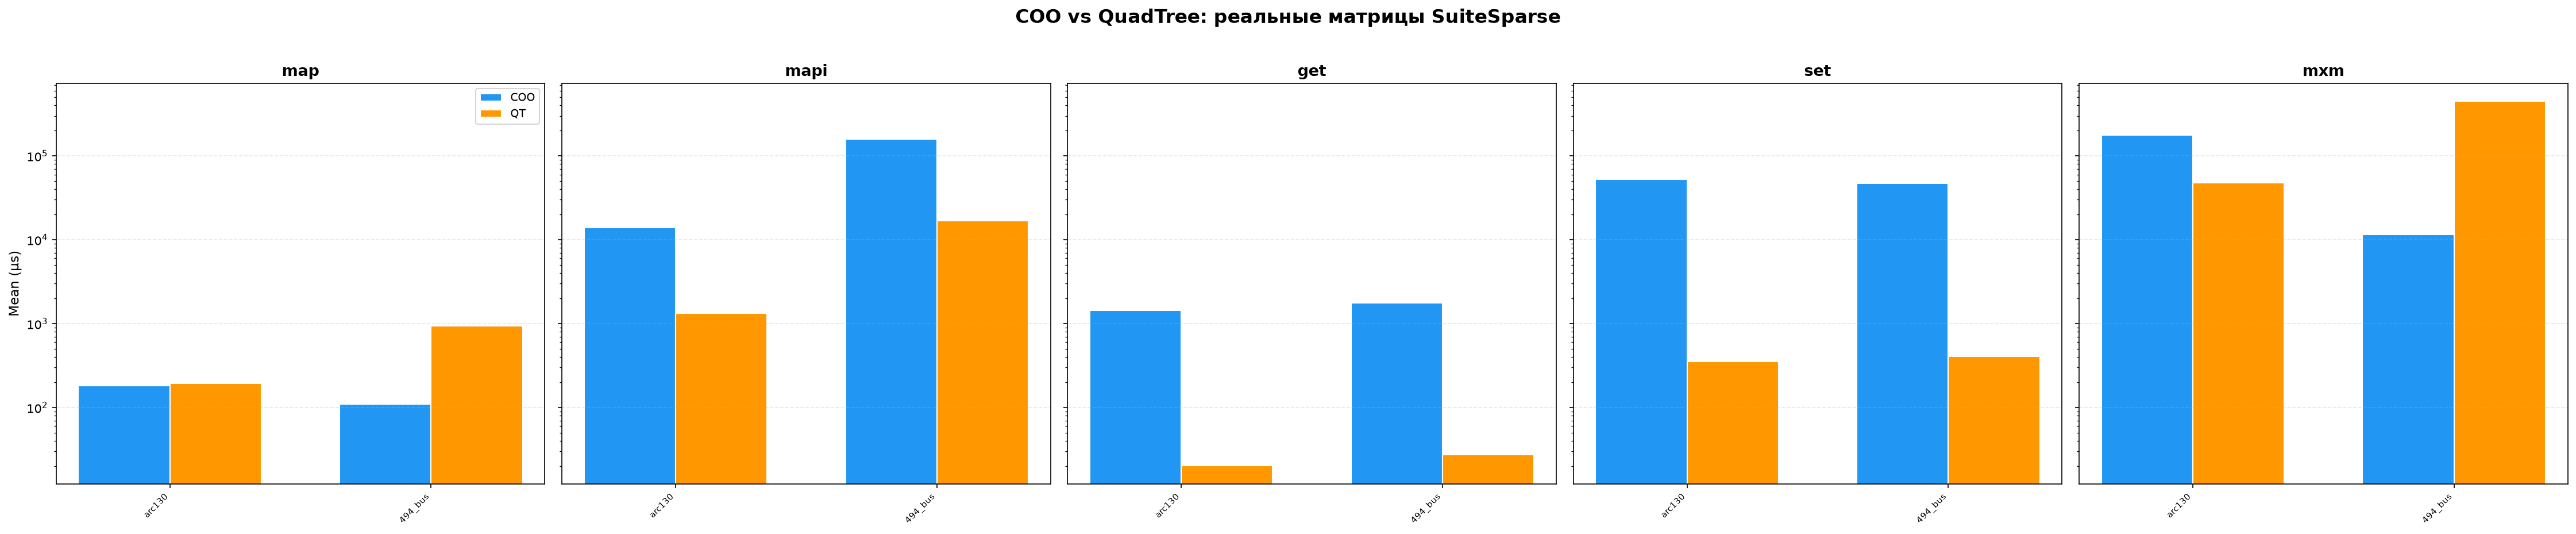
\includegraphics[width=0.98\textwidth]{images/real_summary.png}
    \caption{Сводная диаграмма: время выполнения пяти операций на реальных матрицах (494\_bus и arc130). Левая колонка~--- COO, правая~--- quadtree. Ось~Y~--- время в микросекундах (логарифмическая шкала).}
    \label{fig:real_summary}
\end{figure}

\begin{figure}[H]
    \centering
    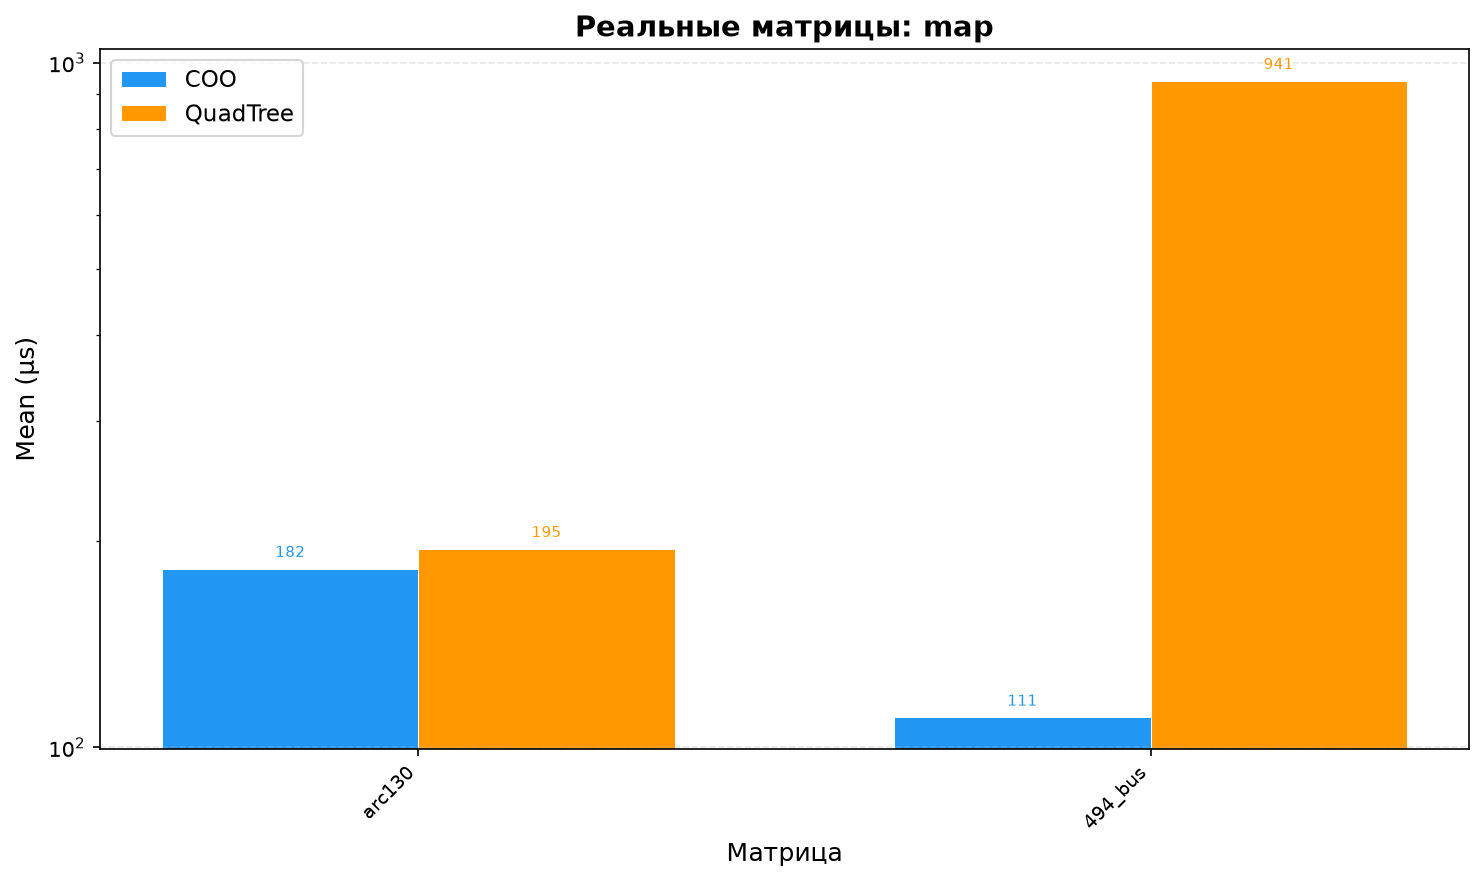
\includegraphics[width=0.92\textwidth]{images/real_map.png}
    \caption{Время выполнения \texttt{map} на реальных матрицах.}
    \label{fig:real_map}
\end{figure}

\begin{figure}[H]
    \centering
    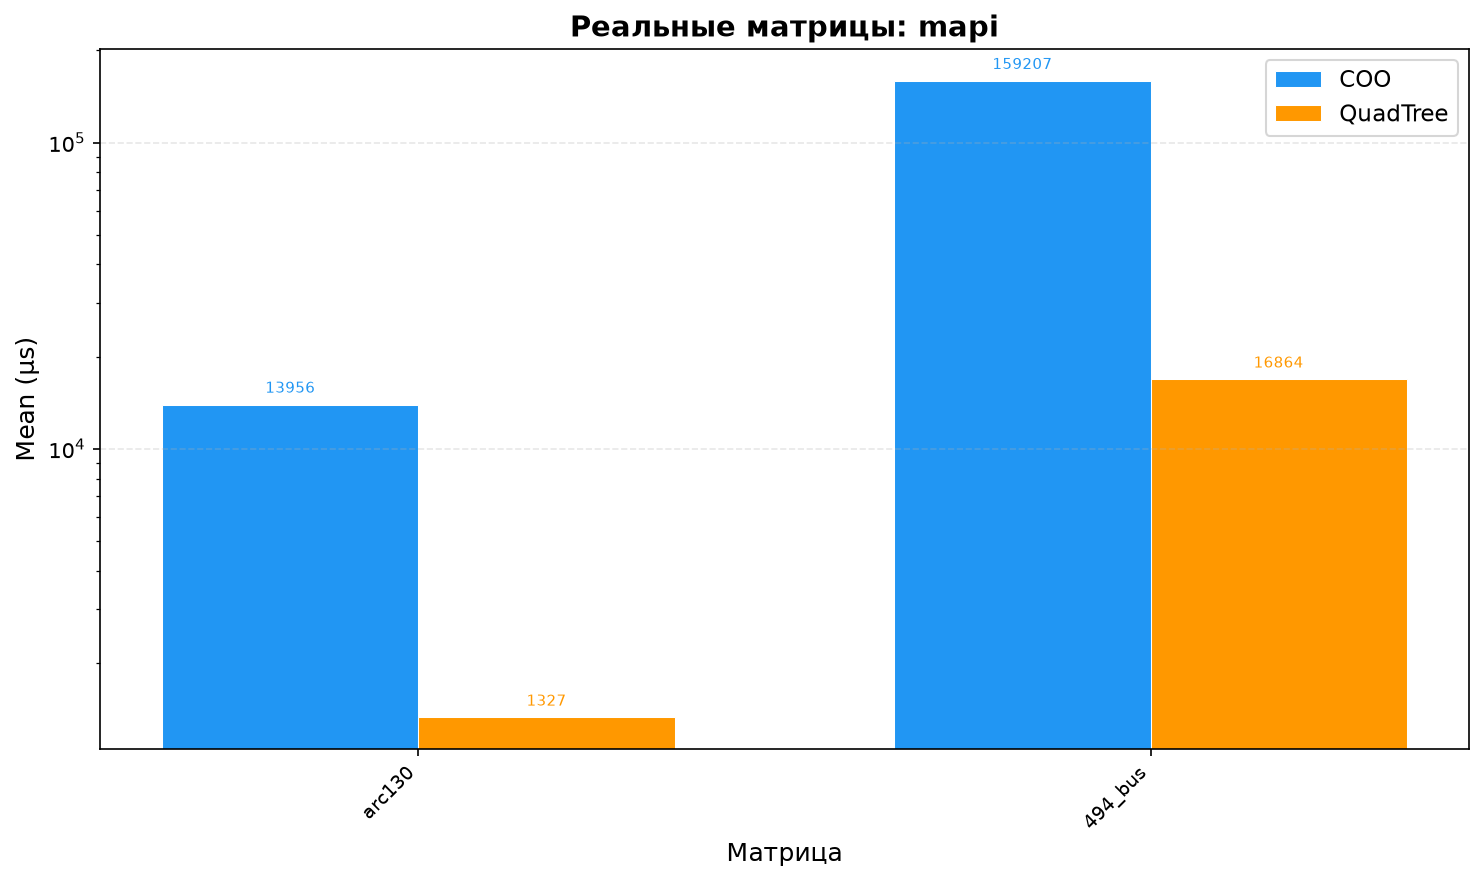
\includegraphics[width=0.92\textwidth]{images/real_mapi.png}
    \caption{Время выполнения \texttt{mapi} на реальных матрицах.}
    \label{fig:real_mapi}
\end{figure}

\begin{figure}[H]
    \centering
    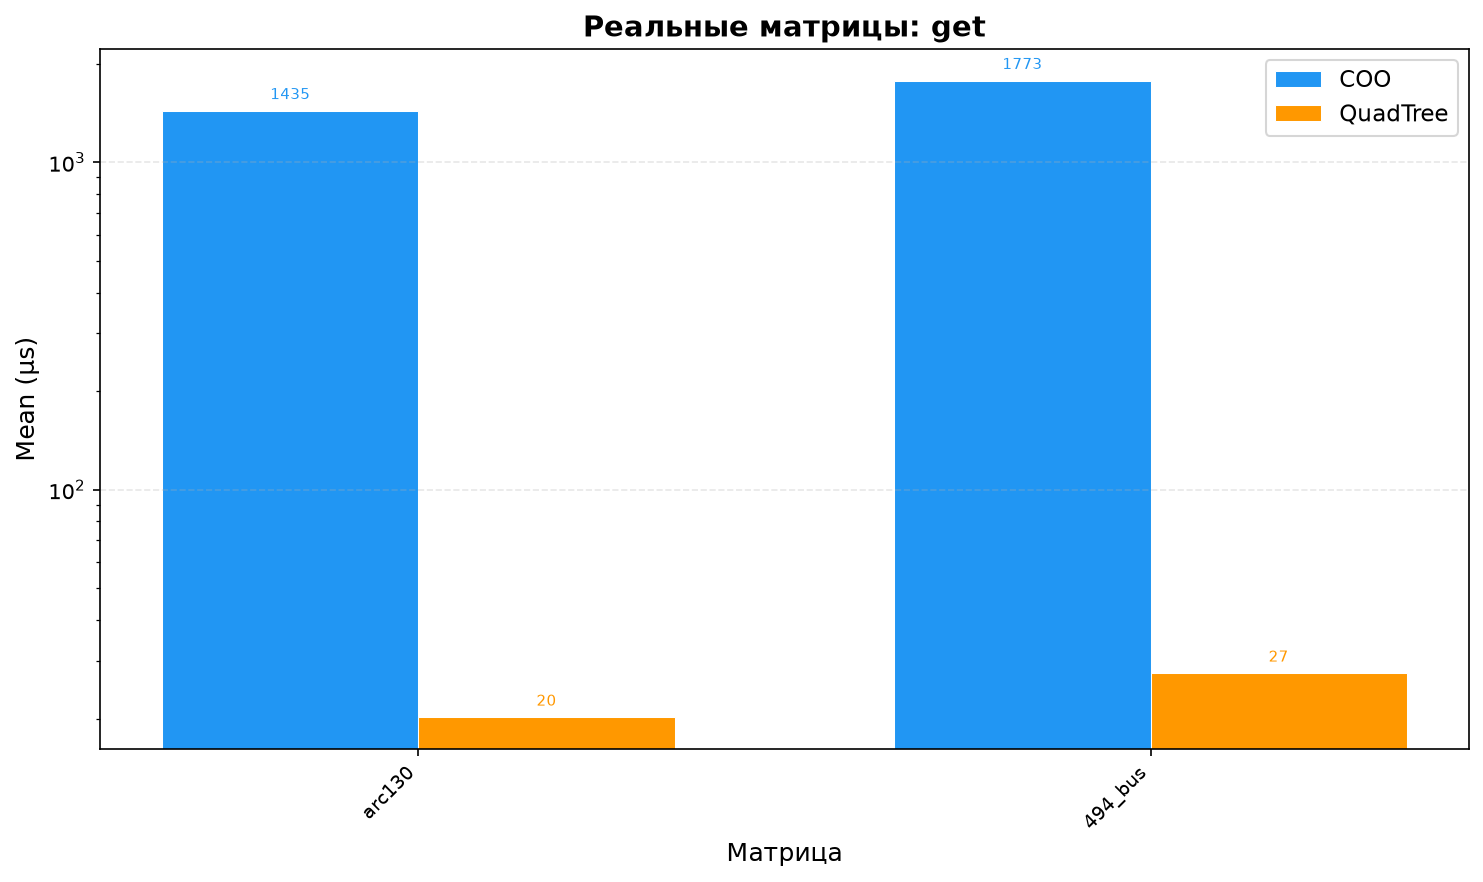
\includegraphics[width=0.92\textwidth]{images/real_get.png}
    \caption{Время выполнения \texttt{get} на реальных матрицах.}
    \label{fig:real_get}
\end{figure}

\begin{figure}[H]
    \centering
    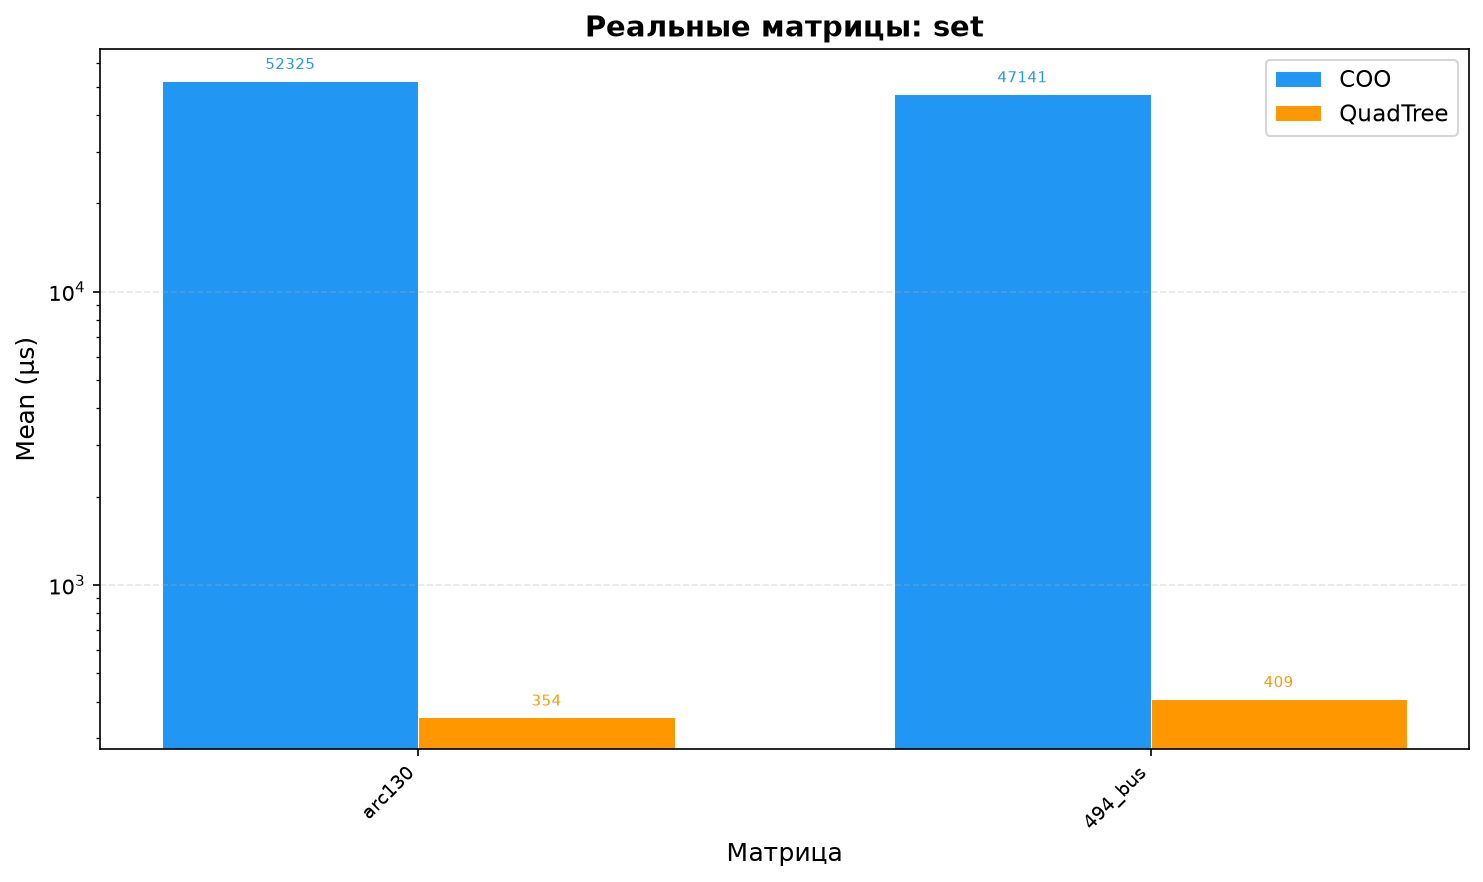
\includegraphics[width=0.92\textwidth]{images/real_set.png}
    \caption{Время выполнения \texttt{set} на реальных матрицах.}
    \label{fig:real_set}
\end{figure}

\begin{figure}[H]
    \centering
    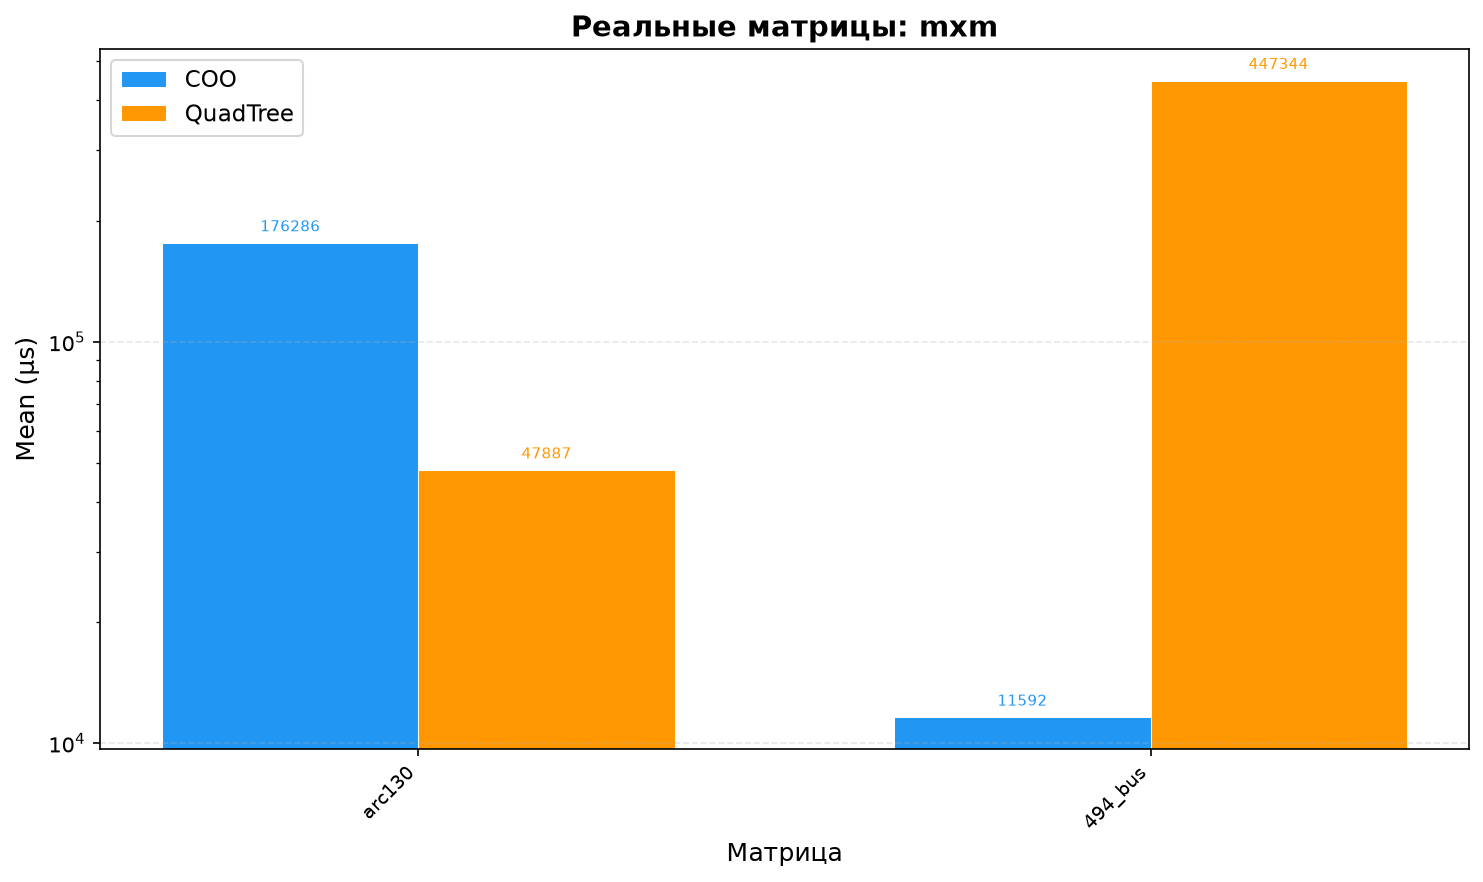
\includegraphics[width=0.92\textwidth]{images/real_mxm.png}
    \caption{Время выполнения \texttt{mxm} на реальных матрицах.}
    \label{fig:real_mxm}
\end{figure}

\section{Анализ асимптотической сложности}

Для каждого формата определена ожидаемая асимптотическая сложность основных операций. Пусть $N$~--- размер стороны матрицы, $n$~--- число ненулевых элементов, $k$~--- глубина дерева ($k = \log_2 N$).

\begin{table}[H]
    \centering
    \caption{Ожидаемая асимптотическая сложность операций}
    \label{tab:complexity}
    \begin{tabular}{lcc}
        \toprule
        Операция & COO & QuadTree \\
        \midrule
        \texttt{get} (доступ)        & $O(n)$      & $O(\log N)$ \\
        \texttt{set} (обновление)    & $O(n)$      & $O(\log N)$ \\
        \texttt{map} (отображение)   & $O(n)$      & $O(T)$      \\
        \texttt{mapi}                & $O(N^2)$      & $O(T)$      \\
        \texttt{map2} (две матрицы)  & $O(n_1 + n_2)$ & $O(T_1 + T_2)$ \\
        \texttt{mxm} (умножение)     & $O(n_1 \cdot n_2 / N)$ & $O(N^{\log_2 8})$ \\
        \bottomrule
    \end{tabular}
\end{table}

Здесь $n$~--- число ненулевых элементов матрицы, $T$~--- число узлов дерева (с учётом конденсации), $n_1$, $n_2$~--- числа ненулевых элементов умножаемых матриц.

Ключевые отличия:

\begin{itemize}
    \item \textbf{Доступ и обновление.} В COO поиск элемента~--- линейный перебор $O(n)$, поскольку тройки хранятся в плоском списке. В quadtree доступ~--- рекурсивный спуск по дереву за $O(\log N)$, что существенно быстрее для разреженных матриц, где $n \gg \log N$.
    \item \textbf{Отображение (map).} COO обходит только $n$ троек, quadtree~--- все $T$ узлов дерева. Если матрица сильно разреженная и дерево сильно сжато ($T \ll N^2$), quadtree может быть быстрее. Если дерево не сжимается (плотные данные), quadtree обходит все $N^2$ элементов.
    \item \textbf{Умножение матриц.} COO использует стратегию «умножение строк на столбцы» с группировкой по строкам: сложность $O(n_1 \cdot \bar{n_2})$, где $\bar{n_2}$~--- среднее число ненулевых элементов в строке второй матрицы. Quadtree использует рекурсивный divide-and-conquer: $O(N^{\log_2 8}) = O(N^3)$ в худшем случае, но с конденсацией поддеревьевреальная сложность может быть существенно ниже.
\end{itemize}

\section{Результаты}

Сводные результаты измерений на реальных матрицах приведены в табл.~\ref{tab:real_results}.

\begin{table}[H]
    \centering
    \caption{Среднее время выполнения операций на реальных матрицах (мкс), усреднённое по 5 независимым запускам (Mean $\pm$ StdDev)}
    \label{tab:real_results}
    \begin{tabular}{lrrrr}
        \toprule
        \multirow{2}{*}{Операция} & \multicolumn{2}{c}{494\_bus} & \multicolumn{2}{c}{arc130} \\
        \cmidrule(lr){2-3} \cmidrule(lr){4-5}
        & COO & QuadTree & COO & QuadTree \\
        \midrule
        map   & $122.4 \pm 17.0$  &   $999.9 \pm 118.3$ &  $136.6 \pm 25.6$  &   $205.0 \pm 8.2$  \\
        mapi  &  $159\,207 \pm 12\,574$  &  $16\,864 \pm 507$  &  $13\,956 \pm 379$  &  $1327 \pm 21$     \\
        get   & $1826 \pm 130$    &  $27.9 \pm 0.85$    & $1455 \pm 63.5$    &  $21.2 \pm 2.3$   \\
        set   & $49\,888 \pm 4130$ &  $459.4 \pm 87.7$  & $53\,340 \pm 2320$ &  $354.9 \pm 9.2$  \\
        mxm   & $11\,813 \pm 350$ & $384\,799 \pm 35\,900$ & $173\,456 \pm 9290$ & $45\,128 \pm 8480$ \\
        \bottomrule
    \end{tabular}
\end{table}

Основные наблюдения:

\begin{enumerate}
    \item \textbf{Операции \texttt{map} и \texttt{mapi}.} COO оказывается быстрее quadtree при операции \texttt{map}: на матрице 494\_bus~--- в 8 раз, на arc130~--- в 1,5 раз. Это согласуется с табл.~\ref{tab:complexity}: COO обходит только список троек ($O(n)$), тогда как quadtree обходит все узлы дерева ($O(T)$). Однако для операции \texttt{mapi} quadtree также оказывается быстрее: на 494\_bus~--- примерно в 9 раз, на arc130~--- примерно в 10,5 раза. Причина в том, что \texttt{mapi} должна обеспечивать общий вид~--- вызывать функцию отображения для всех $N^2$ позиций матрицы (включая пустые), что для COO означает полный перебор $O(N^2)$, тогда как quadtree обходит только узлы с данными ($O(T)$).
    \item \textbf{Операция \texttt{get}.} Quadtree значительно быстрее: на 494\_bus~--- в 65 раз, на arc130~--- в 69 раз. Это соответствует теоретическим ожиданиям: quadtree выполняет доступ за $O(\log N)$ (табл.~\ref{tab:complexity}), тогда как COO~--- линейный перебор за $O(n)$.
    \item \textbf{Операция \texttt{set}.} Quadtree быстрее: на 494\_bus~--- в 109 раз, на arc130~--- в 150 раз. Причина~--- аналогична операции \texttt{get}: обновление в quadtree~--- это $O(\log N)$, тогда как в COO~--- $O(n)$ (вставка в отсортированный список).
    \item \textbf{Умножение матриц (\texttt{mxm}).} Результат зависит от структуры матрицы. На 494\_bus COO быстрее в 33 раза, на arc130~--- quadtree быстрее в 3,8 раза. Алгоритм \texttt{mxmcoo} выполняет группировку по строкам и перебор только ненулевых пар ($O(n_1 \cdot \bar{n_2})$), что эффективно для матриц с умеренной плотностью. Quadtree использует рекурсивный divide-and-conquer алгоритм с восемью умножениями подматриц, что хорошо работает для матриц с чёткой блочной структурой.
\end{enumerate}

\section{Заключение}

В ходе выполнения работы получены следующие результаты.

\begin{itemize}
    \item Реализован модуль COO с операциями доступа, обновления, отображения и умножения матриц в формате Coordinate List.
    \item Реализованы мостовые функции для конвертации между форматами COO и quadtree.
    \item Написаны 133 модульных теста (27~--- для модуля COO), все тесты проходят.
    \item Разработана инфраструктура измерения производительности на базе BenchmarkDotNet с методологией повторных измерений (несколько независимых запусков для оценки воспроизводимости).
    \item Проведён сравнительный анализ производительности форматов COO и quadtree на синтетических и реальных данных.
    \item Установлено, что COO эффективнее для операций \texttt{map} и \texttt{mxm} (при определённых условиях), тогда как quadtree эффективнее для \texttt{get}, \texttt{set} и \texttt{mapi} за счёт структуры дерева, обеспечивающей $O(\log N)$ доступ и обход только узлов с данными.
\end{itemize}

\begin{thebibliography}{99}
    \bibitem{qtreefsharp} Репозиторий QTreeFSharp. URL: \url{https://github.com/Lamagraph/QTreeFSharp} (дата обращения: 15.07.2026).
    \bibitem{suitesparse} SuiteSparse Matrix Collection. URL: \url{https://sparse.tamu.edu/} (дата обращения: 15.07.2026).
    \bibitem{benchmarkdotnet} BenchmarkDotNet. URL: \url{https://benchmarkdotnet.org/} (дата обращения: 15.07.2026).
    \bibitem{fsharpdocs} F Sharp Programming. URL: \url{https://en.wikibooks.org/wiki/F_Sharp_Programming} (дата обращения: 15.07.2026).
    \bibitem{matplotlib} Matplotlib documentation. URL: \url{https://matplotlib.org/stable/contents.html} (дата обращения: 15.07.2026).
\end{thebibliography}

\section{Репозиторий}

Исходный код проекта: \url{https://github.com/narysh/QTreeFSharp}

\end{document}
